\section{Program Logic for Location Virtualization}
\label{sec:logic}
% The predicate gen_heap_interp.
\newcommand{\gammaPred}{\delta}
\newcommand{\gammaPreds}{\delta\textsf{s}}
\newcommand{\rtv}{\textsf{rtv}}
\newcommand{\qone}{\texttt{q1}}
\newcommand{\qtwo}{\texttt{q2}}
\newcommand{\qthree}{\texttt{q3}}
\newcommand{\qfour}{\texttt{q4}}

\newcommand{\sumwalkabs}[3]{
  \ownGhost\gammaPred{\authfrag{\singletonMap{#1}{(#2, #3)}}}
}

\newcommand{\sumapaces}[2]{
  \ownGhost\gammaPreds{\authfrag{\singletonMap{#1}{#2}}}
}
\newcommand{\ptableabswalk}[1]{\mathcal{A}\textsf{bsPTableWalk}(#1)}
\newcommand{\ptablestore}{\theta}

\add{
  A program logic for reasoning about code which may work with (and possibly update) multiple address spaces requires dealing with
  several key challenges. It must ensure that reasoning about memory accesses only depends on assertions that hold
  in the active address space at the time of access. It must allow invariants for code or data structures to refer
  to other address spaces. These constraints mean it must also support reasoning about when the active address space
  changes, as this affects which memory assumptions are usable or not for memory access and thus which data structures are
  immediately directly accessible.
}
\add{
  Many approaches which could handle these problems in principle, such as tagging pointers with the relevant address space.
  But such approaches introduce other complexities.
  Most code, even in an operating system kernel, only works with a single address space (the current one).
  Explicitly plumbing address space information through a simple linked list specification, simply because some other part of the program
  may manipulate other address spaces, adds significant specification burden.
  Specifications which need to talk about a particular invariant holding in a specific other address space (or multiple other address spaces) would need to quantify
  over \emph{functions} from address space identity to assertions rather than just assertions.
  Using a modal approach resolves all of these challenges cleanly and uniformly.
  Specifications that are not \emph{about} address space manipulation need not mention an address spaces at all:
  one can use standard separation logic data structure specifications without restructuring,
  and every assertion can be stated for either the current or specific other address spaces.
  In short, modalities make it possible for specifications to mention address spaces when necessary,
  without requiring mention when only one address space is at hand.
}

We describe a program logic (a separation logic) along the lines suggested \replace{earlier}{above}, where every assertion is relative
to an address space in which it is interpreted, allowing us to define \emph{virtual points-to} assertions that make claims
about memory locations in a particular address space. Virtual addresses, and even virtual points-to assertions, 
are not tagged with their address spaces in any way. Memory access in this logic is validated through the use
of virtual points-to assertions in preconditions, which guarantee that address translations succeed.
This supports rules for updating not only typical data in memory that happens to be subject to address translation, but \add{also}
manipulation of the page tables themselves via virtual addresses (as demanded by all modern hardware) \replace{also}{and}
via virtual points-to assertions.
To support specifications that deal with multiple address spaces, our logic incorporates a hybrid-style modality
$[r](P)$ to state that an assertion is true in another (assertion-specified) address space rather than the address space
currently active in hardware, which is not only useful for virtual memory manager invariants, but \add{also} critical to reasoning
about change of address space.
By developing this within the \iris framework, we obtain additional features (e.g., fractional permissions) that allow us to verify
some of the most subtle and technically challenging instruction sequences in an OS kernel (Section \ref{sec:experiment}).



% We derive a program logic (a separation logic) supporting the following stances and constraints:
% \begin{enumerate}
% \item \textit{address spaces as modal contexts}: Assertions in our logic are context-dependent,
%   in the sense that their truth depends on which address space they are used in, due to the need to support virtual points-to assertions.
% \item \textit{sharing}: The physical location backing a virtual address's storage is located (during a page table walk) through a 
%       set of physical page-table (L4-L1 page-tables) acceses that are shared amongst different virtual addresses (specifically,
%       those on the same page of memory\footnote{of in the case of L2 or higher levels of tables, within a given broader region.}).
%       This sharing imposes constraints on defining points-to assertions
%       in terms of physical (L4-L1) page-table memory accesses
% \item \textit{context-agnostic-resources}: each virtual address is valid under a certain address space, 
%       but it does not represent this \textit{knowledge} of its address space. 
%       That is, assertions are not explicitly tagged with their address space validity
% \item \textit{updating address-space mappings}: We present logical abstractions to enable 
%       updating not only pages of typical data in memory, but also page tables themselves.\footnote{Prior work relied on unfolding operational semantics
%       to verify page table updates.}
% \item \textit{explicitly-modal assertions}: Our logic includes a means to talk about facts being true
%       in another address space
% \item \textit{address-space switch as changing the "World" of truth}: Switching from one address-space to another logically
%       becomes a simultaneous introduction-and-elimination of a pair of modal assertions (for different address spaces)
% \end{enumerate}

% The idea that the truth of an assertion is relative to an address space has far-reaching consequences.
To support making assertions depend on a choice of address space, we work entirely in a pointwise lifting of \iris's base BI logic,
essentially working with separation logic assertions indexed by a choice of page table root as a $\mathcal{W}_{64}$, which we call $\textsf{vProp }\Sigma$:\footnote{
  \iris experts may notice our \lstinline|-b>| resembles another pointwise lifting already in  \iris~\cite{dang2019rustbelt,dang2022compass}. 
  This similarity is real, but the existing lifting does not appear to work with indexed \coq types like our \lstinline|word n| as a domain.
}
\lstinline[language=Coq]|Definition vProp  $\Sigma$ : bi := word 64 -b> iPropI  $\Sigma$|.
This is the (\rocq) type of assertions in our logic.
Most constructs in \iris's base logic are defined with respect to any BI-algebra (of \coq type \lstinline|bi|), so \add{they} automatically
carry over to our derived logic.
% \add{Since \textsf{vProp}s are ``just'' \textsc{Iris} predicates on a choice of page table root,\todo{this section may be subsumed under first addition to this section, don't need both}
% it may not be obvious what the gain is over simply using \textsc{Iris} directly.
% The gain is not expressive power.
% Every modal logic can be translated straightforwardly to a logic without modalities
% (nearly always a small variation on the \emph{standard translation} from propositional modal logic
% to first-order logic~\cite{blackburn2006modal}\footnote{\add{Itself similar to verification condition generation
% for weakest precondition calculi and Hoare logics.}}) that can directly address the logic's models ---
% but these translations, in addition to making specifications far more verbose,
% generally do not preserve the appealing reasoning principles of modal logics.
% This becomes \replace{most}{more} apparent when discussing our proof rules.
% }
However, we must still build up from existing \iris primitives to provide new primitives that depend on the address space --- primarily the notion
of virtual points-to.
To define and use virtual points-to assertions, we require two basic assertions that ignore
the current address space:

\paragraph{Register points-to} 
The assertion $\textsf{r}\;\mapsto_{\textsf{r}}\{q\}\;\textsf{rv}$ ensures the ownership of the register $\rg$ containing the
value of the register $\rv$.
The fraction $\qfrac$ with value 1 asserts the unique ownership of the register mapping and grants update permission \replace{on}{to} it;
otherwise, any value $0 < \qfrac <1$ represents partial ownership, granting read-only permission on the mapping.\footnote{
\add{We adopt the standard naming convention of $\qfrac$-related names representing fractional permission, with fractions
sometimes appearing in braces or as subscripts in various asertions.}}

\paragraph{Physical memory  points-to} The soundness proofs for our logic's rules largely center around
proving that page-table-walk accesses as in Figure \ref{fig:pagetables} succeed, which requires assertions
dealing with physical memory locations.
We have two notions of physical points-to facts. The primitive notion closest to our machine model is captured by an assertion
$ \textsf{pfn} \ \sim \ \textsf{pageoff} \mapsto_{\textsf{a}} \; \{\textsf{q}\} \; \textsf{v} $, where \textsf{pfn} (a $\mathcal{W}_{52}$ \emph{page frame number}) essentially selects a 4KB page of physical memory,
and \textsf{pageoff} (a $\mathcal{W}_{12}$) is an offset within that page.
% could be an 52-bits masked address to level 4 table 
% ($\textsf{w1 } =( \textsf{ l4M52 maddr cr3val}) $),
%and, expectedly \textsf{w2} is an address computed by page-offset computation (e.g. $\textsf{l4off maddr cr3val}$). 
From this we can derive a more concise physical points-to when the split is unimportant:
% Giving a raw 64-bits memory pointsto assertion becomes
{$\textsf{w} \mapsto_{\textsf{p}} \{q\} \textsf{ v} \stackrel{\triangle}{=} (\textsf{drop 12}~w) \ \sim \ (\textsf{bottom 12}~w)\mapsto_{\textsf{a}} \; \{\textsf{q}\} \textsf{ v} $}

 %I put a newline in between the following two Definitions as the second Definition seems not proper without the newline
\begin{figure*}
  \begin{lstlisting}[language=Coq,escapeinside={(*}{*)}]
 Definition $\vaddr\mapsto_{\textsf{t}}\{\textsf{q}\}\; \vpage$ : vProp $\Sigma$ := 
  $\exists_{\textsf{l4e l3e l2e l1e}} \ldotp$  $\ulcorner$ aligned $\vaddr \urcorner \ast$ L4_L1_PointsTo($\vaddr$ l4e l3e l2e l1e paddr) $\ast$ paddr $\mapsto_{p}\{\mathsf{q}\} \vpage$.
 Definition L4_L1_PointsTo (maddr l4e l3e l2e l1e paddr :word 64) : vProp $\Sigma$ := $\lambda$ cr3val.
  $\ulcorner$ entry_present l4e $\land$ entry_present l3e $\land$ entry_present l2e $\land$ entry_present l1e$\urcorner$ $\ast$
  (l4M52 maddr cr3val) $\sim$ (l4off maddr cr3val) $\mapsto_{a}$ {q1}  l4e  $\ast$(*\label{line:l4pointsto}*)
  (l3M52 maddr l4e) $\sim$ (l3off maddr l4e)  $\mapsto_{a}$ {q2}  l3e $\ast$(*\label{line:l3pointsto}*) 
  (l2M52 maddr l3e) $\sim$ (l2off maddr l3e) $\mapsto_{a}$ {q3}  l2e $\ast$(*\label{line:l2pointsto}*)
  (l1M52 maddr l2e) $\sim$ (l1off maddr l2e) $\mapsto_{a}$ {q4}  l1e $\ast$ $\ulcorner$ addr_L1(va,l1e) = paddr $\urcorner$.(*\label{line:l1pointsto}*)
\end{lstlisting}
\vspace{-1em}
\caption{A Strong Virtual Points-to Relation
}
  \label{fig:strongvirtualpointsto}
\vspace{-1em}
\end{figure*}



\subsection{An Overly-Restrictive Definition for Virtual Memory Addressing}
\label{sec:overly-restrictive}
A natural definition for a virtual points-to
asserting that virtual address \textsf{va} points to a value \textsf{v}
would 
% require that in order for a virtual address \textsf{va} to point to a value \textsf{v}, the assertion 
contain
partial ownership of the physical memory involved in the page table walk that would translate \textsf{va} to
its backing physical location --- with locations existentially quantified since a virtual points-to should not assert
\emph{which} locations are accessed in a page table walk, as in Figure \ref{fig:strongvirtualpointsto}.
It asserts the existence of four page-table entries, one at each translation level, and via \lstinline|L4_L1_PointsTo|
asserts that the physical page table walk (per Figure \ref{fig:pagetables}) succeeds in reaching the L1 entry,
which points to the page holding the physical memory backing the virtual address, which contains value \textsf{v}.
Most of the definition lives directly in \textsf{vProp}, using the separation logic structure lifted from \iris's \textsf{iProp}.
\looseness=-1

\lstinline|L4_L1_PointsTo| works by
chaining together the entries for each level, using the sequence of table offsets from the address being translated to index
each table level, and using the physical page address embedded in each entry.\footnote{
  The fractions \lstinline|q1| through \lstinline|q4| represent the fractional ownership of each entry based on how many
  word-aligned addresses might need to share the entry ---  $(\frac{1}{512})^n$ for each level $n$.
}
For example, the first-level address translation to get the L4 entry (\lstinline|l4e|) 
  uses the masks \textsf{l4M52} with the current \lstinline|cr3| to get the physical address of the start of the L4 table
  and \textsf{l4off} with the virtual address being translated to compute the correct \add{byte} offset within that table \add{just as in the first translation
  step of Figure \ref{fig:pagetables}}.\footnote{\add{Note the offsets mentioned in Figure \ref{fig:pagetables} are 9-bit indexes into the 512 entries; the byte offset is that times 8.}}
  \replace{
    Then {at} that physical location {is} the appropriate entry in the L4 table \textsf{l4e}.
  }{
    Thus Line \ref{line:l4pointsto} asserts that the physical address built from the table base and offset points to the L4 entry \textsf{l4e}.
  }
  Subsequent levels of the page table walk \add{assertion (Lines \ref{line:l3pointsto}--\ref{line:l1pointsto})} work similarly.
The statement of these assertions is simplified by the use of our split physical points-to assertions, since
each level of tables is page-sized. \footnote{We do not address superpages and hugepages in this paper.}
This helper definition is also more explicit in \textsf{vProp} which binds a value to \lstinline|cr3| and uses it to start the translation process.
\looseness=-1


% Given the definition of physical page-pointsto assertion and the root address of virtual-address space as shown in Figure \ref{fig:pagetable}, one can build the physical address-translation for a virtual address (e.g. \textsf{va}) via abstracting the L4-L1 table traversal as the following:
% \begin{itemize}
%   \item Level-4 Translation (L4): Performs 
%   the first level address translation to get the L4 entry (L4E) in Figure \ref{fig:pagetables} by using the masks l4M52 and l4off with \textsf{rtv} virtual base address to get the starting address of the L4 table (L4T), and locate the entry amongst 512 (q1) ones respectively.
%     \begin{lstlisting}[language=Coq]
%       $\hbox{(\TirNameStyle{{L4translate}})} \quad$ (l4M52 maddr rtv) \$\sim$\ (l4off maddr rtv) $\mapsto_{a}$ {q1} l4e 
%     \end{lstlisting}
%  \item Level-3 Translation (L3): Performs the second level address translation to get the L3 entry (L3E) in Figure \ref{fig:pagetables} by using the masks l3M52 and l3off with L4 entry (l4e) to get the starting address of the L3 table (L3T), and locate the entry amongst 512 ones (q2) respectively.
%     \begin{lstlisting}[language=Coq]
%     $\hbox{(\TirNameStyle{{L3translate}})}$ (l3M52 maddr l4e) \$\sim$\ (l3off maddr l4e)  $\mapsto_{a}$ {q2} l3e
%     \end{lstlisting}
%   \item Level-2 Translation (L2): Performs the second level address translation to get the L2 entry (L2E) in Figure \ref{fig:pagetables} by using the masks l2M52 and l2off with L3 entry (l3e) to get the starting address of the L2 table (L2T), and locate the entry amongst 512 ones (q3) respectively.
% \begin{lstlisting}[language=Coq]
%     $\hbox{(\TirNameStyle{{L2translate}})}$ (l2M52 maddr l3e) \$\sim$\ (l2off maddr l3e)  $\mapsto_{a}$ {q3} l2e
%     \end{lstlisting}
%   \item Level-1 Translation (L1): Performs the second level address translation to get the L1 entry (L1E) in Figure \ref{fig:pagetables} by using the masks l1M52 and l1off with L2 entry (l2e) to get the starting address of the L1 table (L1T), and locate the entry amongst ones 512 (q4) respectively.
%    \begin{lstlisting}[language=Coq]
%     $\hbox{(\TirNameStyle{{L1translate}})}$ (l1M52 maddr l2e) \$\sim$\ (l1off maddr l2e)  $\mapsto_{a}$ {q4} l1e
%     \end{lstlisting}
%   \item Page Address Level Translation: Final computed physical page-address ($\textsf{addr\_L1}(\vaddr$,$\textsf{l1e}$)) points-to the value stored in the address ($\vpage$).
%    \begin{lstlisting}[language=Coq]
%     $\hbox{(\TirNameStyle{{PageLevelAccess}})} \qquad$ addr_L1($\vaddr,\textsf{l1e}$) $\mapsto_{p} \vpage$.
%     \end{lstlisting} 
% \end{itemize}

This solution is in fact very close to that of \citet{kolanski08vstte}, who define a separation logic from scratch in \textsc{Isabelle/HOL},
where the semantics of all assertions are functions from pairs of heaps and page table root values to booleans.\footnote{
  This was a typical explicit construction at the time; their work significantly predates \iris.
}
Our solution \replace{removes}{in the next subsection improves on theirs, removing} some restrictions in this definition by further abstracting the handling of address translation.
\looseness=-1

\subsection{Aliasing/Sharing Physical Pages}
  \label{sec:sharingpages}  
  The virtual points-to definition shown in Figure \ref{fig:strongvirtualpointsto} 
  is too strong to specify some operations that a virtual memory manager may need to do, such as move one level of the page table to a different physical location while preserving all virtual-to-physical mappings. %\footnote{
  %   x86-64 hardware, like other architectures, includes a feature (which we do not formalize assertions for) to
  %   replace an L1 page table address in an L2 entry with a pointer to a \emph{larger} 2MB page (called super-pages), 
  %   or replace an L2 page table address in an L3 entry with a pointer to a 1GB page (called huge-pages).
  % }
  The use of $\textsf{L}_{4}\_\textsf{L}_{1}\_\textsf{PointsTo}$ in Figure \ref{fig:strongvirtualpointsto}'s
  virtual points-to definition stores knowledge of the page table walk details with ownership of the backing physical memory.
  Updating any of these mappings (e.g., moving the page tables in physical memory, as in coalescing for superpages or hugepages)
  would require explicitly collecting all virtual points-to facts that traverse affected entries.
  It is preferable to permit the page tables themselves to be updated independently of the virtual points-to assertions,
  so long as those updates preserve the same virtual-to-physical translations.
  But this is not possible with Figure \ref{fig:strongvirtualpointsto}'s definition, which ties ownership of particular pieces of page table memory to the virtual points-to.


  % iris.sty lacks nice syntax for the ghost maps
  \newcommand{\ghostmaptoken}[3]{\ensuremath{#2\hookrightarrow^{#1}#3}}
  \newcommand{\fracghostmaptoken}[4]{\ensuremath{#2\hookrightarrow^{#1}_{#4}#3}}

\newcommand{\vale}{\textsf{val}}
\begin{figure*}
\footnotesize
\centerline{$
\begin{array}{l}
    \vaddr\mapsto_{\textsf{v}}\{\textsf{q}\}\;\vale : \mathsf{vProp}~\Sigma \stackrel{\triangle}{=} 
    \exists \paddr\ldotp
    \exists \delta\ldotp
    % \underbrace{(\lambda\mathit{cr3val}\ldotp\sumapaces{\mathit{cr3val}}\delta)}_\text{Find addr.\;space invariant} \ast 
    \underbrace{(\lambda\mathit{cr3val}\ldotp\exists \epsilon\ldotp\fracghostmaptoken{\delta{}s}{cr3val}{\delta}{\epsilon})}_\text{Find addr.\;space invariant} \ast 
  % \underbrace{\sumwalkabs\vaddr\qfrac\paddr }_\text{Ghost translation}\ast 
  \underbrace{\fracghostmaptoken{\delta}{\mathsf{va}}{\mathsf{pa}}{\mathsf{q}} }_\text{Ghost translation}\ast 
  \underbrace{\paddr \mapsto_{\mathsf{p}}\{\textsf{q}\}\; \vale}_\text{Physical location}
\end{array}
$}
\vspace{-1em}
\caption{Virtual-Points-to for Sharing Pages}
  \label{fig:virtualpointstosharing}
\end{figure*}  

  % Intuitively, the definition in Figure \ref{fig:strongvirtualpointsto} is too strong because the virtual points-to
  % assertion there tracks too much information: when writing programs that access memory via virtual addresses,
  % most code does not care \emph{which physical memory locations are involved in address translation}: it only cares
  % that virtual address translation would succeed. The necessary information about the physical page table walk
  % must still be tracked, but can be tracked separately from the virtual points-to assertion itself.
  % In practice the decisions about which virtual addresses are valid rest not with code posessing a virtual address, but with
  % the virtual memory manager --- and its invariants.

  \begin{figure}
\footnotesize
\vspace{-1em}
  \begin{mathpar}
  \inferrule*[right=\footnotesize GhostMapUpdate]{ }{\mathsf{GhostMap}(\gamma,\theta) \ast \ghostmaptoken{\gamma}{\mathsf{pa}}{\mathsf{va}} \vs 
  \mathsf{GhostMap}(\gamma,\theta[\mathsf{va}\mapsto\mathsf{pa'}]) \ast \ghostmaptoken{\gamma}{\mathsf{va}}{\mathsf{pa}'} 
  }
  \and
  \inferrule*[right=\footnotesize GhostMapLookup]{ }{\mathsf{GhostMap}(\gamma,\theta) \ast \ghostmaptoken{\gamma}{\mathsf{va}}{\mathsf{pa}} \wand \ulcorner \theta(\mathsf{va})=\mathsf{Some}(\mathsf{pa}) \urcorner }
  \end{mathpar}
\vspace{-2em}
  \caption{\iris rules for ghost maps}
  \label{fig:ghostmaps}
  \end{figure}

  We separate the physical page-table walk from the virtual points-to relation, replacing it with a ghost state that merely guarantees that the address translation would succeed.
  \iris includes a \emph{ghost map} construction, which we use to track mappings from virtual addresses to the physical addresses they translate to as a piece of ghost state.
  The map includes, for each key in the map (i.e.,
  each virtual address), a token $\ghostmaptoken{\gamma}{k}{v}$ whose ownership is required to update that key-value pair in the ghost map named $\gamma$. The existence of such a token implies that the actual map $\theta$ tracked by a corresponding $\mathsf{GhostMap}(\gamma,\theta)$
  resource indeed maps $k$ to $v$. These properties are captured by key \iris rules in Figure \ref{fig:ghostmaps}.\footnote{\iris ghost maps lack established notation\add{;}
  \del{in the literature, but} the syntax we use captures the details of \texttt{iris.base\_logic.lib.ghost\_map}.}
  There are other rules, but these two are most important for explaining ghost maps.
  \textsc{GhostMapUpdate} says that ownership of the actual ghost map with ghost name $\gamma$ and map contents $\theta$,
  and a \del{full (non-fractional) }token witnessing that $\theta$ maps \textsf{pa} to \textsf{va} permits an update to the ghost map's state,
  changing the map and replacing the token to represent the new value.
  \textsc{GhostMapLookup} allows using the same information to simply conclude that the mapping indicated by the token is true.
  
  The \emph{virtual memory manager's invariant} ensures that for each $\ghostmaptoken{\gamma}{\vaddr}{\paddr}$ mapping in this map, there are \emph{physical} resources sufficient to ensure that the address translation for $\vaddr$
will resolve on the hardware to $\paddr$ --- via $\textsf{L}_{4}\_\textsf{L}_{1}\_\textsf{PointsTo}$.
  \add{This kernel invariant turns out to be a key ingredient in supporting proofs of VMM functionality:
  in Section \ref{sec:experiment} we will see that separating the logical and physical virtual-to-physical mappings
  is what allows stating the global kernel invariants needed for software page traversals, which prior work did not (and could not) pursue.}
  \looseness=-1

  %Thus the specification of \emph{which} physical addresses support translation is separated from the virtual points-to.
  % But these physical resources, which specify \emph{which} physical locations
  %are involved in the page table walk, are now separated from but consistent with
  %the knowledge that such resources exist (which is embodied by the token for $va$, which tracks that $va$ maps to $pa$
  %in the ghost map). Thus we can store the token which summarizes the translation and ensures it exists in the virtual
  %points-to, and keep the ghost map and the invariant that every mapping in the ghost map has corresponding physical resources
  %for translation in a separate global invariant for each address space.

  % In Iris this is realized by using an authoritative resource algebra: there is a single \emph{authoritative} global copy of the (ghost)
  % map caching virtual-to-physical address translations, and for each entry a read only \emph{partial} ownership of that key-value pair.
  % The resource algebra itself is instantiated as:
  % \[\mathcal{A}\textsf{bsPTableWalk} \stackrel{\triangle}{=} \textsc{Auth} (\; \mathcal{W}_{64} \;\rightarrow_{\textrm{fin}} \;  ( (\textsc{Frac }, \mathord{+}) \times (\textsc{Agree } \Loc,\mathord{=}) ))\]
For clarity, we refer to the specific ghost map summarizing virtual-to-physical translations by 
\mbox{$\mathcal{A}\textsf{bsPTableWalk}(\delta,\theta) \stackrel{\triangle}{=} \mathsf{GhostMap}(\delta,\theta)$}
(omitting $\delta$ for brevity when only one is in scope)
and keep this in a per-address-space invariant described shortly.
We then replace the physical traversal $\textsf{L}_{4}\_\textsf{L}_{1}\_\textsf{PointsTo}$ in Figure \ref{fig:strongvirtualpointsto}'s virtual points-to definition
with ownership of the token \ghostmaptoken{\delta}{\vaddr}{\paddr}, %ghost-map ($ \sumwalkabs\vaddr\qfrac\paddr$),
yielding Figure \ref{fig:virtualpointstosharing}'s definition.
This new definition guarantees that the ghost map \add{$\theta$} \replace{contains an mapping from}{maps} the virtual address ($\vaddr$) to a physical address ($\paddr$),
and thus that the per-address-space invariant \add{described next} will contain the physical resources that guarantee \add{that} the hardware resolves the translation.
\looseness=-1

  \begin{figure*}
  \footnotesize
\vspace{-1em}
\centerline{$
\begin{array}{l}
  \mathcal{I}\textsf{ASpace}(\ptablestore,m)\stackrel{\triangle}{=} \textsf{ASpace\_Lookup}(\ptablestore,m) \ast 
  \bigast{(\vaddr, \textsf{pa})\in \ptablestore}{\exists\;(\textsf{l4e l3e l2e, l1e, pa})\ldotp \textsf{L}_{4}\_\textsf{L}_{1}\_\textsf{PointsTo}(\vaddr\textsf{, l4e, l3e, l2e, l1e, pa})} \\
  \textsf{ where } 
   \textsf{ASpace\_Lookup} (\ptablestore,m) \stackrel{\triangle}{=} \lambda\textsf{ cr3val} \ldotp \; \exists \gammaPred \; \ldotp \ulcorner m \; !!\; \textsf{cr3val} = \textsf{Some } \gammaPred \urcorner \ast
    %\ownGhost\gammaPred{\authfull{\ptableabswalk\ptablestore}}
    \ptableabswalk{\delta,\theta}
\end{array}
$}
\vspace{-1em}
\caption{Per-address-space invariant with a fixed global map of address space names $m$}
  \label{fig:peraspaceinvariant}
\vspace{-1em}
  \end{figure*}

We place the authorative ownership of the ghost \add{map} translation $\mathcal{A}\textsf{PTableWalk}$ in a per-address-space invariant
$\mathcal{I}$\textsf{ASpace} (Figure \ref{fig:peraspaceinvariant}), 
\replace{$\mathcal{I}$\textsf{ASpace} alone allows}{allowing} changes to the page tables
that preserve overall virtual-to-physical translations \add{in isolation},
\add{and also allowing changes to specific the virtual-to-physical translations}
\replace{W}{w}hen combined with the
\replace{fragment}{token} stored in the \add{relevant} virtual points-to (Figure \ref{fig:virtualpointstosharing}).
\del{changes in the virtual-to-physical translations become possible without the need to track all virtual points-to assertions.}
\looseness=-1

% \todo[inline,color=cyan]{Explain $\delta{s}$ (Iris ghost name) vs $m$ (logical contents of ghost map) in next 2 paragraphs}
% \todo[inline]{This next paragraph below explains details, but should first explain the big picture: the current address space
% is identified by a paddr, so to state the invariant for the address space named by that paddr we need to look up
% what invariants should hold, then assert that those invariants do hold.}
\add{We must also ensure that different address spaces can have independent ghost maps ---
which we resolve with an additional unique global ghost map (with ghost name $\delta{s}$) from address-space identifiers (page table roots
whose values are manipulated by the kernel code) to
the \textsc{Iris} ghost name for that address space's ghost map.
In Figure \ref{fig:virtualpointstosharing}, the extra ghost map token for $\delta{s}$ asserts that $\delta$ --- which is exisentially
quantified --- is the correct ghost name for the current address space. That is then the ghost map named
in the ghost virtual-to-physical translation token of Figure \ref{fig:virtualpointstosharing}.
}
\del{In Figure ??,
$\theta$ is the logical map from virtual addresses to the physical addresses they should translate to, 
for the \emph{current} address space, corresponding to the  currently installed page tables (the ones
indicated by \texttt{cr3}). In Figure ??, the existentially quantified $\delta$
is the ghost name for this map (again, for the current address space).
Because our logic is the first to address the existence of multiple address spaces,
it must ensure that $\theta$ actually corresponds to the intended ghost map for the current address space.
This requires looking up the ghost name (i.e., $\delta$) for the current address space,
which is handled by $m$ --- another logical map (tied to ghost state shortly)
from various page table roots to ghost names for the per-address-space ghost maps discussed above.
}
\add{
Just as the ghost name $\delta$ names the ghost map with contents $\theta$,
$\delta{s}$ names a ghost map, whose contents appear as $m$ in Figure \ref{fig:peraspaceinvariant} (the association of $\delta{s}$ to $m$
is a global invariant not shown).
}
$\mathcal{I}\textsf{ASpace}(\theta,m)$ then \add{performs 3 roles:
it associates the current address space's root with an appropriate \textsc{Iris} ghost name $\delta$;
it tracks authoritatively that $\delta$'s logical contents match $\theta$; and it}
stores the physical resources for the current address space mappings \add{(via the iterated $\textsf{L}_{4}\_\textsf{L}_{1}\_\textsf{PointsTo}$)}.
\del{ensuring that the current address space is valid (has an entry in $m$ whose corresponding
authoritative map matches $\theta$), and asserting ownership of the appropriate fractional ownership
of the physical page table walk for each virtual-to-physical translation in $\Theta$ (for the current address space).}

\del{
Virtual points-to assertions must also ensure that they are tied to a valid address space, and because they
use ghost map tokens to ensure the virtual-to-physical translation exists in a specific ghost map, they must also
name that map. In Figure \ref{fig:virtualpointstosharing}, this is done with a ghost map token for \emph{another} ghost map,
one shared across the kernel, holding $m$. Our virtual points-to assertion existentially quantifies the address-space-specific
ghost map $\delta$ mapping virtual addresses to physical addresses, and ensures it exists with a token for the distinguished
global (unique) ghost map named by $\delta{s}$.}
% the ghost map of virtual-to-physical translations for a particular address space (the ghost name $\delta$ in Figure \ref{fig:virtualpointstosharing}).
% % for each address space must be locateable from a representation of the specific address space:
% % This means we also require a way to locate the map for the current address space from 
% We support lookup by the current root page table pointer stored in \lstinline|cr3|.
\looseness=-1
  
% Figure \ref{fig:logicaladdrspace} depicts the relationships between these pieces, for a single
% address space.
% The invariant for the currently active address space (solid round square labelled as 
% $\mathcal{I}$\textsf{ASpace} in Figure \ref{fig:logicaladdrspace}) asserts authorative ownership (i.e. 
% update capability), $\ownGhost\gammaPred{\authfull{\ptableabswalk\ptablestore}}$, of the ghost map $\Theta$
% describing virtual-to-physical address translations
% -- shown as a solid-round-head arrow to $\mathcal{A}\textsf{PTableWalk}$.
% Each virtual points-to assertion (dashed round square labelled as \textsf{Virtual PointsTo}
%  in Figure \ref{fig:peraspaceinvariant})
% asserts fragmental ownership of the ghost map $\Theta$, $\sumwalkabs\vaddr\qfrac\paddr$,
% shown via the dashed-diamond-head arrow to $\mathcal{A}\textsf{PTableWalk}$. Specifically, it asserts that
% the virtual address the virtual points-to assertion concerns corresponds to some physical address.
% There exists only one persistent authorative ownership 
% ($\ownGhost\gammaPred{\authfull{\ptableabswalk\ptablestore}}$) which collects the fragmental 
% ghost page-table-walk mapping ($\sumwalkabs\vaddr\qfrac\paddr$),
%  shown as double-ended solid arrow 1 to N imposing the update protocol.

% \begin{figure}
%    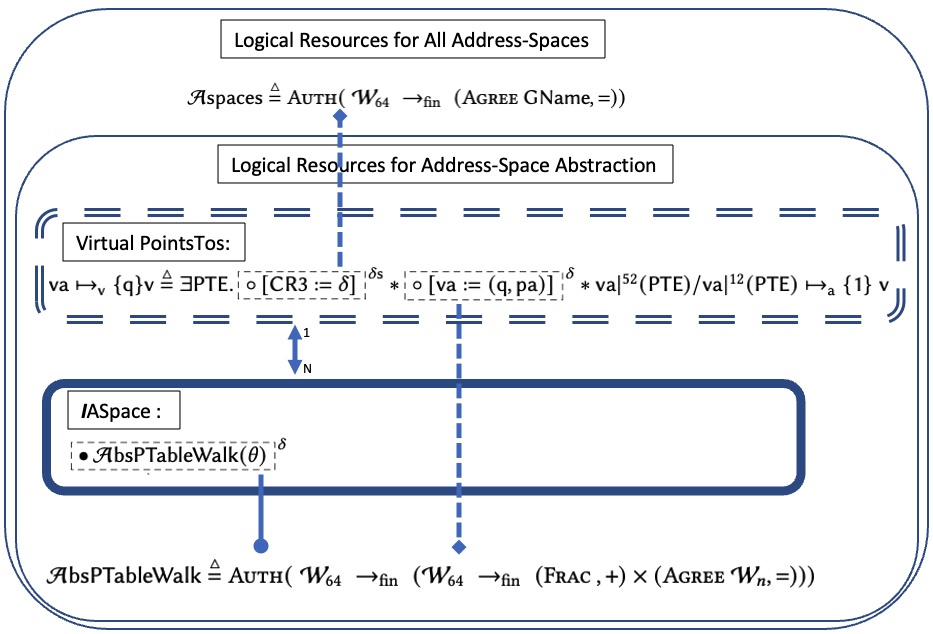
\includegraphics[width=0.75\columnwidth]{logical_addr_space.png}
%   \caption{Logical Resources of Address-Space Abstraction (1 Address Space)}
%   \label{fig:logicaladdrspace}
%   \end{figure}

% \paragraph{From A Single Address Space to Many}
% In principle the resources from each individual address space should be collected into a single
% shared invariant, and for each memory access,
% a fragment of this corresponding to $\mathcal{I}\textsf{ASpace}(\Theta,m)$
% for the current address space should be extracted from this global resource, used to prove correctness of the
% memory access, and put back.
% In this paper we focus on the middle section, explicity identifying resources for each
% address space. The reason for this is that in practice, this global resource is also
% the place where kernel-specific assumptions, such as guaranteeing that certain virtual address range
% was mapped in all address spaces, would be enforced. This paper focuses on the
% reasoning principles behind the virtual memory access, and we leave the use of this within a larger
% kernel to future work. We do, however, deal with the existence of multiple address spaces in examples (Section \ref{sec:experiment}).

\subsection{Address Space Management}
\label{sec:aspacemanagement}
% So far, we have introduced logical abstractions for a single address space, but VMMs
Real VMMs must
 handle more than one address space.
Doing so requires a way to talk about other address spaces, and means to switch address spaces.
\begin{figure}
\footnotesize
\[\begin{array}{c}
    \mbox{$[r](\mathsf{P}) \;: \mathsf{vProp} \; \Sigma \; \stackrel{\triangle}{=} \; \lambda \_,\; \mathsf{P}~\mathsf{r} \vspace{0.5em}$}
    \qquad
    \mbox{$\textsf{Fact P} \stackrel{\triangle}{=} \;\forall \; ,r \; r' \ldotp  \textsf{P r} \dashv\vdash \textsf{P r'}$}
    \qquad
    \inferrule*{ }{\textsf{Fact}\;[r](\textsf{P}) }
    \qquad
    \inferrule*{ }{\textsf{Fact}\;(\textsf{r}\;\mapsto_{\textsf{r}}\{q\}\;\textsf{rv})}
    \\[1.3em]
    \inferrule{ }{\textsf{Fact}\;(\textsf{w} \mapsto_{\textsf{p}} \{q\} \textsf{ v} )}
    \qquad
    \inferrule{ }{(\textsf{P} \vdash \textsf{Q}) \vdash  ([r](\textsf{P}) \vdash  [r](\textsf{Q}))}
    \qquad
    \inferrule{ }{[r](\textsf{P} \ast \textsf{Q}) \dashv\vdash ([r](\textsf{P}) \ast [r](\textsf{Q})}\vspace{0.5em}
    \\[1.3em]
    \inferrule{ }{[r](\textsf{P}\land \textsf{Q}) \dashv\vdash [r](\textsf{P})\land [r](\textsf{Q})}
    \qquad
    \inferrule{ }{[r](\textsf{P}\lor \textsf{Q}) \dashv\vdash [r](\textsf{P})\lor [r](\textsf{Q})}
    \qquad
    \inferrule{ }{\textsf{Fact P} \vdash  [r](\textsf{P}) \dashv\vdash (\textsf{P})} %(\textsf{vProp }\Sigma))\\
\end{array}\]
\vspace{-1em}
  \caption{Other-space Modality and Its Laws}
  \label{fig:modaldef}
\vspace{-1em}
  \end{figure}
Figure \ref{fig:modaldef} gives the definition of our modal operator for asserting the truth of a modal
(address-space-contingent) assertion \emph{in another address space}, which we call
the \emph{other-space} modality. The definition itself is not
particularly surprising --- as our modal assertions are semantically predicates on a page table root (physical)
address, the assertion $[r](P)$ is a modal assertion that ignores the (implicit) current page table root,
and evaluates the truth of $P$ as if $r$ were the page table root. 
The novelty here is not in the details of the definition, but in recognizing that this is the right way to deal with
multiple address spaces, and working out how to support interaction of multiple address spaces (discussed in the next section).
\add{The modal assertions, together with the other-space modality, mean we can give generic definitions
of data structure assertions (e.g., linked lists, etc.) which do not need to track information
about their own address space. In fact, \emph{only} assertions that explicitly deal with multiple address
spaces need to mention address spaces at all (via the other-space modality).
}

We can prove that this modality follows certain basic laws, showing that its truth is independent of the address
space in which it is considered, \add{that} it distributes over various logical connectives, and \add{that} it follows the rule of
consequence.
We call \textsf{vProp} assertions whose truth is independent of the current address space
\textsf{Fact}s; these include other-space assertions, physical memory points-tos, and register assertions.
\textsf{Fact}s can \add{freely} move in and out of other address space modalities\del{ freely}.
\looseness=-1

In general, per-address-space invariants should be collected in a larger
VMM invariant, with individual address spaces' invariants pulled out as needed, such as when proving
soundness of an individual virtual memory access.
\replace{But}{However,} such larger invariants would contain many kernel-specific properties that are orthogonal
to the fundamental reasoning principles that are the focus of this paper.
We leave such kernel-specific reasoning to future work, but our verification of task switching
(Section \ref{sec:experiment}) demonstrates support for managing multiple address spaces.
\looseness=-1



  
% \begin{figure}
% \[
% \begin{array}{l}
%   \{ \textsf{cr3 } \mapsto_{r} R0 \ast a_0 \mapsto_{\textsf{v}}p_0  \ast a_1 \mapsto_{\textsf{v}}p_1  \ast [r1]\;( b_0 \mapsto_{\textsf{v}}p_3  \ast b_1 \mapsto_{\textsf{v}}p_4 )\}\\
%   \qquad \qquad \qquad \qquad \qquad \mathsf{mov\_ctl} \;\; \texttt{cr3} \; \; R1\\

%   \{ \textsf{cr3 } \mapsto_{r} R1 \ast [r0](a_0 \mapsto_{\textsf{v}}p_0  \ast a_1 \mapsto_{\textsf{v}}p_1)  \ast  b_0 \mapsto_{\textsf{v}}p_3  \ast b_1 \mapsto_{\textsf{v}}p_4 \}
%   \end{array}
% \]
%   \label{fig:addrswitch}
%   \end{figure}

% \begin{remark}[The Choice of Modal Context, Contingency and  Pattern of Verification Context]
%   \label{remark:pattern}
% The truth on an address space, exhibits itself as a contingent truth: a location virtualization assertion (a virtual points-to in \ref{fig:virtualpointstosharing}),  happens to valid in the \textit{current world} (in the current address space), and switching address spaces pulls information out of one \textit{world} into the “current view” of memory, and leaves other assertions true relative to the previous address space.

% Therefore, an address-space, as an abstraction, can be treated as naming the memory state as a modal frame and the choice of page table root as a world in Kripke-style semantics. Not suprisingly, transition between two address-spaces, then, can be just an entailment relation \textit{alternating} the \textit{named-state}

% Being inspired by what hybrid logic \ref{} calls a satisfaction operator, which evaluates the truth of a predicate in a named alternative state (here, address space), we give a modal definition describing the truth of assertions for the resources (i.e. virtual pointsto relations) inside the address space. Ignoring the predicate types for a while, $[r]P$ in Figure \ref{fig:modaldef}, indicates that $P$ holds in the virtual address space rooted at $r$, the truth ($P$) on an address-space is indexed by the root page-table address $r$ of the address-space. In the rest of this section, we explain the structural aspects -- the modal resource context of address space modality -- , and how we lift the interaction of address-space modality with the ambient logic, i.e. separation logic as an entailment for specifying \textit{address-space-switch}.

% Pragmatically, 
%   \begin{enumerate}
%   \item a modal context with its context-resources and picked contingency defines a modality (e.g. a address-space modality $[r]P$). For the convenience of verification, it enables focusing on the certain facts in the interest of reasoning (e.g. virtual pointsto relations in the current address-space)
%   \item and, offloads the burden of individual bookkeeping of these facts (e.g. virtual pointsto relations per address-space) under different context (e.g. virtual pointsto relations in other address-spaces) via utilizing the \textit{summarization} aspect of the contingency it represents (e.g. other virtual pointsto relations are valid under other certain address-space page-table root addresseses).  
%   \end{enumerate}
% \end{remark}




\subsection{Selected Logical Rules}
\label{sec:selected_rules}
% Per the discussion in Section \ref{sec:issues}, w
As common for assembly-level verification~\add{\cite{Ni2006codeptrs,ni2007contexts}}, we define our logic using Hoare doubles:%\footnote{This
% omits some low-level Iris details (stuckness, observations) that play no meaningful
% role in our development.}
\\\centerline{$
  \begin{array}{l}
    %\textsf{wpd\_def e s E1 } \Phi \;\mathsf{ rtv } : \textsf{iProp }\Sigma := \\
    \{ \Phi \}_\mathsf{ rtv }\;\textsf{e} : \textsf{iProp }\Sigma := 
   % \qquad
   ((\textsf{cr3} \mapsto_{\textsf{r}} \textsf{rtv} \ast \Phi) \textsf{ rtv}) \wand \textsf{WP e } \{\_, \textsf{True} \}
    \end{array}
$}\\
Our Hoare doubles $\{\Phi\}_\textsf{rtv}\;\textsf{e}$ state that the expression (i.e., sequence of instructions)
\textsf{e} are safe to execute (will not fault)
when executed with \textsf{vProp} precondition $\Phi\ast\textsf{cr3}\mapsto_{\textsf{r}} \textsf{rtv}$.
\textsf{WP} is \iris's own weakest precondition modality, unmodified~\cite{jung2018iris}.
Making \textsf{rtv} a parameter to the double (vs.\ a simple register assertion)
makes it possible to ensure ownership of the \lstinline|cr3| register and its value is accounted for
while avoiding some technical headaches with trying to enforce that $\Phi$ itself contains that.
\looseness=-1
% solves a technical problem with ensuring that the page table root used to evaluate
% the \textsf{vProp} (i.e., evaluating the assertion in the \emph{current}) address space
% is feasible.
% \footnote{Consider the difficulty of selecting the correct page table root value from an arbitrary
% opaque $\Phi$, which may even existentially quantify the page table root. An alternative is to
% require $\Phi$ to have a syntactic form where we can directly extract the value of \lstinline|cr3|,
% but this makes using Iris Proof Mode (IPM)~\cite{Krebbers:2017:IPH:3009837.3009855} with \textsf{vProps}
%   difficult; IPM works for any type matching the signature of an Iris \lstinline|bi|, which includes
%   \textsf{vProp}s, but manually guiding IPM to put an assertion in a specific position over and over adds
%   significant proof burden.
% }

The rest of this section describes specifications of three key \textsf{AMD64} instructions 
in our logic. 
These rules and others (e.g., including accessing memory at an instruction-specified offset from a register
value, which is common in most ISAs)
can be found in our artifact.
% Each rule in Figure \ref{fig:wpdamd}, 
% is annotated with a root (i.e., \lstinline|cr3|) address value (\textsf{rtv}), 
% under which the resources mentioned in the specification are valid.
In general, we use metavariables $\textsf{r}_s$ and $\textsf{r}_d$ to specify source and destination registers
for each instruction, and prefix various register value variables with \textsf{rv}.
We sometimes use $\textsf{r}_a$ to emphasize when a register is expected to hold an address used
for memory access, though the figure also uses typical assembler conventions of specifying
memory access operands by bracketing the register holding the memory address.
Standard for Hoare doubles, there is a frame resource $P$ in each rule for passing resources
not used by the first instruction in sequence through to subsequent instructions.
Our rules include tracking of each instruction's memory address to track \lstinline|rip| updates, which is critical
for control transfer instructions. Our development also includes handling of the \lstinline|rflags| register updates from arithmetic instructions.
Most rules are otherwise standard (e.g., \lstinline|mov| between registers, etc.), with Figure \ref{fig:wpdamd} showing the rules
most unique to our development.
\add{As a reminder, in systems of Hoare doubles, an instruction's precondition appears in the conclusion of the rule,
and an instruction's ``postcondition'' appears as the precondition to subsequent instructions in the
antecedent of the rule.}
\looseness=-1

\begin{figure}
  \footnotesize
  \makeatletter % allow us to mention @-commands
\def\arcr{\@arraycr}
\makeatother
\begin{mathpar}
%  \inferrule[AddRegImm]{
%  \{P \ast r_d \mapsto_{r} \textsf{rvs} \ast r_s \mapsto_{r}\{q\} \textsf{ rvs} \}_{\textsf{rtv}}\;\overline{ is}
%}{
%  \{P \ast r_d \mapsto_{r} \textsf{rvd} \ast r_s \mapsto_{r}\{q\} \textsf{ rvs} \}_{\textsf{rtv}}
%  \textsf{ mov}~\textsf{r}_d,~\textsf{r}_s;\;\overline{is}
%  \lstinline|mov %cr3, r| 
%}
%\\
% \inferrule[WriteToPhysMemFromReg]{
%   \{P \ast r_s \mapsto_{r}\{q\}  \textsf{rvs}  \ast r_a \mapsto_{r} \{q\} \textsf{ vaddr} \ast \textsf{vaddr} \mapsto_{\textsf{t}} \textsf{v} \}_{\textsf{rtv}}\;\overline{ is}  
% }{
%   \{P \ast r_s \mapsto_{r}\{q\}  \textsf{rvs}   \ast r_a \mapsto_{r}\{q\} \textsf{ vaddr} \ast \textsf{vaddr} \mapsto_{\textsf{t}} \textsf{rvs} \}_{\textsf{rtv}}
%   \textsf{ mov}~[\textsf{r}_a],~\textsf{r}_s;\;\overline{is}
% }
% \\
 % \inferrule[AddRegImm]{
 %   \{P \ast\textsf{rip} \mapsto_{\textsf{r}} \textsf{iv+7} \ast  \ast (r_d \mapsto_{r}  \textsf{rvd+imm} \lor  r_d \mapsto_{r} 0 ) \ast r_a \mapsto_{r} \{q\} \textsf{ vaddr} \ast \textsf{vaddr} \mapsto_{\textsf{t}} \textsf{v} \}_{\textsf{rtv}}\;\overline{is}
 % }{
 %   \left\{
 %   \begin{array}{l}
 %   P \ast \textsf{rip} \mapsto_{\textsf{r}} \textsf{iv} \ast \textsf{rflags} \mapsto_{\textsf{r}} \textsf{flgs} \ast \ulcorner (\textsf{rvd + imm} > 0 \lor \textsf{rvd + imm} = 0 ) \urcorner \ast \arcr
 %   r_d \mapsto_{r}  \textsf{rvd} \ast r_a \mapsto_{r} \{q\} \textsf{ vaddr} \ast \textsf{vaddr} \mapsto_{\textsf{t}} \textsf{v}
 % \end{array}\right\}_{\textsf{rtv}}  \;
 %   \textsf{add}~\textsf{r}_d,~[\textsf{imm}];\;\overline{is}
 % }
 % \\
\inferrule[\footnotesize WriteToRegFromVirtMem]{
  \left\{ \begin{array}{l}
    P \ast \mathcal{I}\textsf{ASpace}\ast  \textsf{rip} \mapsto_{\textsf{r}} \; {\textsf{iv} + \textsf{MovLen}(\textsf{r}_d,[\textsf{r}_a])} \ast \arcr
    r_d \mapsto_{r}  \textsf{ v} \ast r_a \mapsto_{r} \; \{q\} \textsf{ vaddr} \ast \textsf{vaddr} \mapsto_{\textsf{v}} \;\{q\} \textsf{ v}
  \end{array} \right\}_{\textsf{rtv}}\;\overline{is}
}{
  \{P \ast \mathcal{I}\textsf{ASpace}\ast \textsf{rip} \mapsto_{\textsf{r}} \textsf{ iv} \ast r_d \mapsto_{r}  \textsf{ rvd} \ast r_a \mapsto_{r} \;\{q\} \textsf{ vaddr} \ast \textsf{vaddr} \mapsto_{\textsf{v}} \textsf{ v} \}_{\textsf{rtv}}\;
  \textsf{mov}~\textsf{r}_d,~[\textsf{r}_a];\;\overline{is}
}
\\
\inferrule[\footnotesize WriteToVirtMemFromReg]{
  \{P \ast \mathcal{I}\textsf{ASpace}\ast \textsf{rip} \mapsto_{\textsf{r}} \textsf{ iv} + \textsf{MovLen}(\textsf{r}_d,[\textsf{r}_a])  \ast r_s \mapsto_{r}\;\{q_1\}  \textsf{ rvs}  \ast r_a \mapsto_{r} \; \{q_2\} \textsf{ vaddr} \ast \textsf{vaddr} \mapsto_{\textsf{v}} \textsf{ v} \}_{\textsf{rtv}}\;\overline{ is}  
}{
  \{P \ast \mathcal{I}\textsf{ASpace}\ast \textsf{rip} \mapsto_{\textsf{r}} \textsf{ iv} \ast r_s \mapsto_{r} \;\{q_1\}  \textsf{ rvs}   \ast r_a \mapsto_{r} \; \{q_2\} \textsf{ vaddr} \ast \textsf{vaddr} \mapsto_{\textsf{v}} \textsf{ rvs} \}_{\textsf{rtv}}
  \textsf{ mov}~[\textsf{r}_a],~\textsf{r}_s;\;\overline{is}
}
\\
%\inferrule[WriteToRegCtlFromReg]{
%  \{P \ast r_s \mapsto_{r}\{q\}  \textsf{ rvs}  \}_{\textsf{rvs}} \overline{is}
%}{
%  \{P \ast r_s \mapsto_{r}\{q\}  \textsf{ rvs}   \}_{\textsf{rtv}}
%  \textsf{mov}~\textsf{cr3},~r_s;\;\overline{is}
  %\lstinline|mov %cr3, r| 
%}\\
\inferrule[\footnotesize WriteToRegCtlFromRegModal]{
  \{[\textsf{rtv}](P \ast \mathcal{I}\textsf{ASpace})\ast \textsf{rip} \mapsto_{\textsf{r}} \textsf{ iv + 4} \ast \mathcal{I}\textsf{ASpace} \ast R\ast r_s \mapsto_{r} \;\{q\}  \textsf{ rvs}  \}_{\textsf{rvs}} \;\overline{is}
}{
  \{P \ast \mathcal{I}\textsf{ASpace} \ast \textsf{rip} \mapsto_{\textsf{r}} \textsf{ iv} \ast [\textsf{rvs}](R \ast\mathcal{I}\textsf{ASpace})\ast r_s \mapsto_{r}\; \{q\}  \textsf{ rvs}   \}_{\textsf{rtv}} \;
  \textsf{mov}~\textsf{cr3},~r_s;\;\overline{is}
  %\lstinline|mov %cr3, r| 
}
% \\
% \inferrule[WriteToRegFromRegCtl]{
%   \{P \ast  \textsf{rip} \mapsto_{\textsf{r}} \textsf{iv + 4} \ast r_d \mapsto_{r} \textsf{rvs} \ast r_s \mapsto_{r}\{q\} \textsf{ rvs} \}_{\textsf{rtv}}\;\overline{ is}
% }{
%   \{P \ast  \textsf{rip} \mapsto_{\textsf{r}} \textsf{iv} \ast r_d \mapsto_{r} \textsf{rvd} \ast r_s \mapsto_{r}\{q\} \textsf{ rvs} \}_{\textsf{rtv}}
%   \textsf{ mov}~\textsf{r}_d,~\textsf{r}_s;\;\overline{is}
%   %\lstinline|mov %cr3, r| 
% }
\end{mathpar}
\vspace{-1em}
\caption{Proof rules for selected \textsf{AMD64} instructions}
\label{fig:wpdamd}
\vspace{-1em}
\end{figure}


\subsubsection{Accessing Virtual Addresses}
Figure \ref{fig:wpdamd} includes two  rules for accessing memory at an address stored in a register $r_a$. 
\add{Setting aside $P$, $\mathcal{I}\textsf{ASpace}$, and the instruction pointer \lstinline|rip|,}
\del{Ultimately, any memory access needs to ensure the relevant address translation would succeed,
which can be ensured by what we informally call the page-table-walk points-to collection
($\textsf{L}_{4}\_\textsf{L}_{1}\_\textsf{PointsTo}$ in Figure ??). }
\TirNameStyle{WriteToRegFromVirtMem} and \TirNameStyle{WriteToVirtMemFromReg}
\del{each use a virtual-pointsto assertion ($\textsf{vaddr} \mapsto_{\textsf{v}} \textsf{v}$),
and }
are nearly-standard (assembly) separation logic rules for memory accesses~\add{\cite{Chlipala2013Bedrock,ni2007contexts}}.
\add{For example, \textsc{WriteToRegFromVirtMem}'s specification
reflects that it reads from the (virtual) memory address \textsf{vaddr} stored in the address
register $\textsf{r}_a$ --- and thus requires register points-to and virtual points-to assertions describing
that relationship and the assumed value \textsf{v} in memory in its precondition (the precondition of the rule's
conclusion). 
It reflects the load (\lstinline|mov|) of that memory value into the destination register $\textsf{r}_d$, with
the updated register points-to in the precondition for $\overline{is}$.
$P$ describes framed resources, which are passed along to the precondition of subsequent instructions,
as in any system of Hoare doubles~\cite{Chlipala2013Bedrock,ni2007contexts}.
\textsc{WriteToVirtMemFromReg} is analogous for writing to memory.
}
\add{There are only two changes specific to our approach.}
\looseness=-1

\replace{However, }{First,}
because we split the physical resources for the page table walk from the
virtual points-to itself (\replace{in order to permit the physical page tables to be freely modified
as long as they preserve virtual-to-physical translations}{per the discussion of Section \ref{sec:sharingpages}}), the rule requires $\mathcal{I}\textsf{ASpace}$
for the current address space to be carried through.
The soundness proofs for these rules extract
the token ($\fracghostmaptoken{\delta}{\vaddr}{\paddr}{\qfrac}$) from the virtual points-to,
use that to extract the physical page-table-traversal points-to collection describing
the page table walk for the relevant address ($\textsf{L}_{4}\_\textsf{L}_{1}\_\textsf{PointsTo}$)
from the invariant ($\mathcal{I}\mathsf{ASpace}$), prove that the page table walk succeeds
and that memory or registers are updated appropriately, before re-packing the invariant and virtual points-to resources.
\looseness=-1

\replace{T}{Second, t}he memory access rules --- as with all rules in our logic ---
\replace{model updates to}{increment} the instruction pointer \lstinline|rip| \add{by the length of the encoded instruction.}
\del{using a metafunction \textsf{MovLen}.}
\textsf{MovLen} returns how long the instruction encoding for the corresponding \lstinline|mov| is;
x86-64 instruction encodings are often longer for instructions using registers that are absent from the 32-bit
x86 ISA that preceded x86-64.
\looseness=-1

\add{Note that the use of a modal abstraction of address space simplifies these rules.
The antecedents of \textsc{WriteToRegFromVirtMem} and \textsc{WriteToVirtMemFromReg}
only mention the address space in the index of the
Hoare double --- not in $P$, or the (virtual) points-to assertions.
There is no extra condition to discharge that the address being accessed is from
the current address space.
}

\subsubsection{Updating \lstinline|cr3|} 
Unlike other rules, \TirNameStyle{WriteToRegCtlFromRegModal} updates the root address of the 
address space determining the validity of resources, from $\rtv$ before the
\lstinline|mov| to $\textsf{rvs}$ afterwards. The global effects of this rule are reflected in moving
\del{bare} assertions \add{for the current address space ($P$ and $\mathcal{I}\mathsf{ASpace}$)} under an other-space modality for \add{the initial
(outgoing) address space} $\rtv$, and moving the new address space's assertions out of
the corresponding modality \add{(since after the \lstinline|mov|, those will hold in the
new current address space)}.

Note that the \emph{global} aspect is important, as a na\"ive frame rule would be unsound for updates to \lstinline|cr3|,
because one could frame out assertions in one address space, switch address spaces, and bring those assertions from the \emph{old}
address space back into the \emph{new} address space, where they may not hold. 
% Appendix \ref{sec:issues} gives more details.
It is often said that the frame rule (below) is one of the key pieces of separation logic.
\centerline{$
  \mbox{$\inferrule*[right=Frame]{
    \{P\}\;C\;\{Q\}
  }{
    \{P\ast R\}\;C\;\{Q\ast R\}
  }$}
  \qquad\begin{array}{c}\textrm{(unsound with address space changes)}\\\\\end{array}
$}\\
Such a rule is normally recoverable from Hoare doubles (see, e.g., \citet{Chlipala2011Bedrock,Chlipala2013Bedrock}).
However, in the presence of address space changes, the traditional frame rule is unsound.
Consider:\\
\centerline{$
  \inferrule*[right=Frame]{
    \inferrule{\ldots }{
    \{\textsf{Pre}\}
    \texttt{mov}~\texttt{\%cr3},~r%\lstinline|mov %cr3, r| 
    \{\textsf{Post}\}
    }
  }{
    \{a\mapsto_\mathsf{v} x \ast \textsf{Pre}\}
    \texttt{mov}~\texttt{\%cr3},~r%\lstinline|mov %cr3, r| 
    \{a\mapsto_\mathsf{v} x \ast \textsf{Post}\}
  }
$}\\
In this (broken!) hypothetical example,
both the precondition and the postcondition assert that $a\mapsto_\mathsf{v} x$ in the current address space, but
\replace{we have no basis for concluding that address translation is preserved by the change of address space}{
  the new address space may map $a$ to another value}. So, this derivation clearly leads to an unsound conclusion. 
The essential problem is that the frame rule is motivated by local reasoning about local updates, but
a switch of address space is a \emph{global} change that may invalidate information about virtual addresses.
Thus, framing around arbitrary \lstinline|cr3| updates is unsound --- hence the \emph{global} nature of \textsc{WriteToRegCtlFromRegModal} ---
though a variant the ensures the same \lstinline|cr3| value is installed before and after the framing
can be recovered.


\subsection{Soundness}
\label{sec:soundness}
Our rules from Figure \ref{fig:wpdamd} are proven to be sound in \iris against an assembly-level hardware model
implementing a fragment of x86-64, including 64-bit address translation with 4-level page tables.
% \todo[inline]{
Our rules for control transfers (\lstinline|jne|, \lstinline|call|, and \lstinline|ret|) are currently
axiomatized (with completely standard specifications~\cite{ni2007contexts,Chlipala2013Bedrock})\footnote{
  \add{An assertion that code at some address is safe to call with a given precondition~\cite{Ni2006codeptrs}
  asserts that the address is mapped and that memory at that address decodes to an instruction sequence
  that is safe with that precondition.
  }
} 
because \iris's built-in machinery does not provide
convenient ways to discard the current continuation; adaptation of others'
approaches~\cite{de2023type} is future work.
Our soundness proofs for all other instructions (including, critically, all memory accesses)
are axiom-free.
% }
% At the moment our proofs do rely on 13 small axioms of properties which should be provable, but
% are challenging to discharge due to some representation choices in our model.\footnote{See \lstinline|srx/x64/machine/current_axioms.v|}
\looseness=-1
